\documentclass{article}

\usepackage{indentfirst}
\usepackage{graphicx}
\usepackage{listings}
\usepackage{fancyhdr}
\usepackage{hyperref}
\usepackage{amsmath}
\usepackage{amssymb}

\title{CIC0097 - Banco de Dados: Projeto \\
        \large \textbf{Tema:} Rede Social}
\author{Guilherme da Rocha Cunha - 221030007 \\
        \and
        Arthur Diehl Barroso - 221029991 \\
        \and
        Eduardo Quirino de Oliveira - 211010305 \\
        \and 
        Breno Costa Avelino Lima - 211010280}
\date{2024.1}

\begin{document}

\pagestyle{fancy}

\maketitle

\begin{figure}[ht]
        \centering
        
\includegraphics[width=.5\textwidth]{imagens/logo_unb.jpg}
\end{figure}

\newpage

\fancyhead{}
\fancyfoot[C]{\thepage}


\renewcommand*\contentsname{Sumário}
\tableofcontents

\newpage

\section{Introdução}
O projeto consiste na aplicação dos conhecimentos adquiridos na disciplina "CIC0097 - Banco de Dados". O banco de dados construído, com o tema Rede Social, utilizou como mecanismo de armazenamento o SQLite e o programa com as funções CRUD foi-se implementado na linguagem Python utilizando o framework web Flask.

\section{Diagrama de Entidade Relacionamento}
\label{sec:mer}
O diagrama abaixo representa o modelo entidade relacionamento do projeto.

\begin{figure}[!ht]
        \centering
        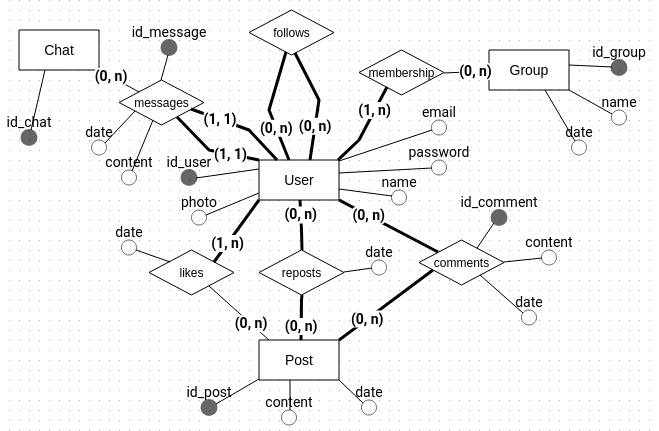
\includegraphics[width=1\textwidth]{imagens/mer.png}
        \caption{Modelo Entidade Relacional}
\end{figure}

\subsection{Entidades}
\subsubsection{User}
\paragraph{Definição:} Representa um usuário no sistema.
\begin{itemize}
        \item Atributo chave: \verb|id_user|.
        \item Atributos simples: \verb|email|, \verb|password|, \verb|name| e \verb|photo|.
\end{itemize}

\subsubsection{Post}
\paragraph{Definição:} Uma publicação feita por um usuário.
\begin{itemize}
        \item Atributo chave: \verb|id_post|.
        \item Atributos simples: \verb|content| e \verb|date|.
\end{itemize}

\subsubsection{Group}
\paragraph{Definição:} Um grupo composto de usuários, similar à grupos do Facebook, comunidades do Orkut e dentre outros.
\begin{itemize}
        \item Atributo chave: \verb|id_group|.
        \item Atributos simples: \verb|name| e \verb|content|.
\end{itemize}

\subsubsection{Chat}
\paragraph{Definição:} Local de conversa entre dois usuários.
\begin{itemize}
        \item Atributo chave: \verb|id_chat|.
\end{itemize}

\subsection{Relacionamentos}
As entidades se relacionam de 6 maneiras distintas:
\begin{enumerate}
        \item Likes: um usuário pode curtir $n$ publicações e uma publicação pode ser curtida por $n$ usuários. Post tem participação total na relação, isto é, toda publicação é feita por algum usuário, mas nem todo usuário faz uma publicação (participação parcial).
        \item Reposts: um usuário pode repostar $n$ publicações e uma publicação pode ser repostada por $n$ usuários. Ambas as entidades têm participação parcial no diagrama.
        \item Comments: um usuário pode fazer $n$ comentários em uma publicação e uma publicação pode ter $n$ usuários comentando. Cada comentário possui sua própria identificação.
        \item Follows: relacionamento recursivo onde um usuário pode seguir $n$ usuários.
        \item Membership: um usuário pode fazer parte de $n$ grupos e um grupo pode ter $n$ membros, onde cada grupo tem que ter pelo menos um usuário que faz parte dele.
        \item Messages: relacionamento ternário entre dois usuários e um chat, onde um usuário pode ter $n$ conversas com outros usuários e um chat pertence a um par de usuários.
\end{enumerate}

\section{Modelo Relacional}
Abaixo encontra-se o modelo relacional gerado a partir do \hyperref[sec:mer]{modelo entidade relacionamento}, utilizando os tipos de dados do SQLite.

\begin{figure}[!ht]
        \centering
        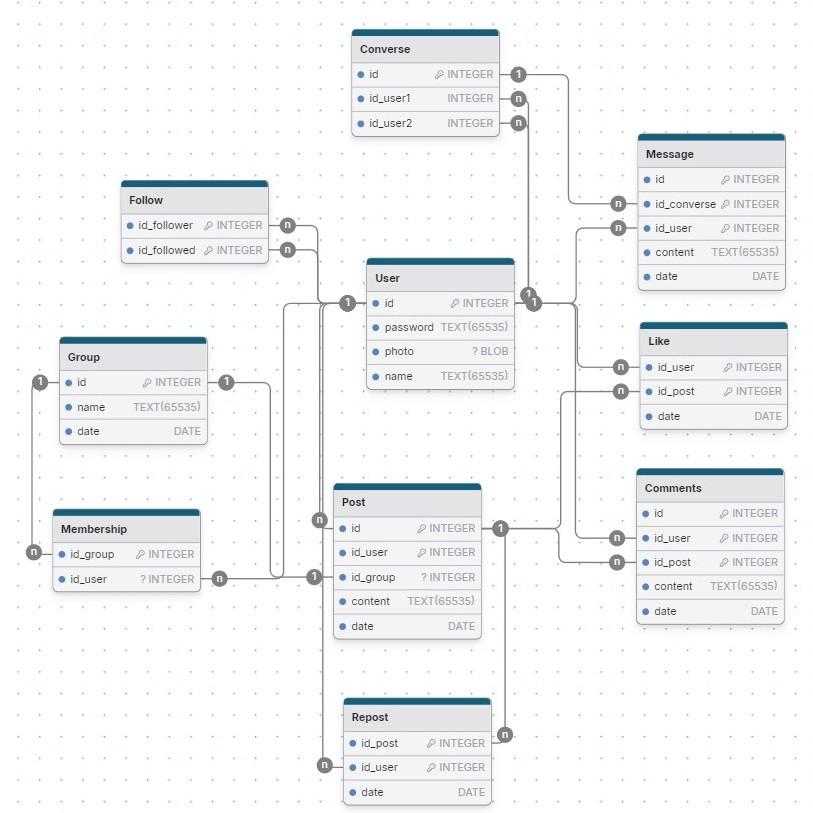
\includegraphics[width=1\textwidth]{imagens/mr.jpg}
        \caption{Modelo Relacional}
\end{figure}

\section{Consultas em Álgebra Relacional}

\section{Avaliação das formas normais}
Analisando as formas normais das tabela, obtemos os seguintes resultados:
\subsection{Primeira Forma Normal}
A tabelas \verb|Post|, \verb|Comments| e \verb|Message| estão na Primeira Forma Normal visto que os atributos do complemento das chaves candidatas não são totalmente funcionalmente dependentes de suas respectivas chaves, isto é, há dependências parciais.

Em todos os casos, como cada tabela possui um \verb|id_<tabela>| como chave primária, os demais componentes das chaves compostas são desnecessários.

\subsection{Segunda Forma Normal}
Nenhuma tabela está na Segunda Forma Normal.

\subsection{Terceira Forma Normal}
A demais tabelas estão na Terceira Forma Normal visto que todas estão na Segunda Forma Normal e não possuem dependências transitivas.

\section{Diagrama da Camada de Mapeamento}
\begin{figure}[!ht]
        \centering
        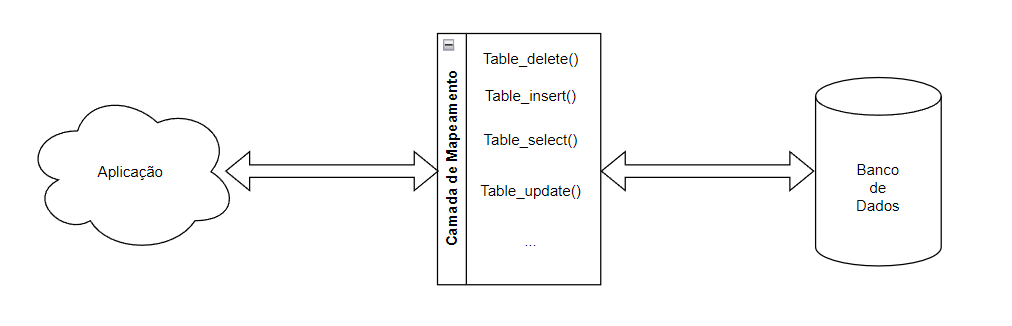
\includegraphics[width=1\textwidth]{imagens/mapeamento.png}
        \caption{Camada de Mapeamento}
\end{figure}

\section{Referências}
\begin{itemize}
        \item ELMASRI, R., NAVATHE, S. B., Sistemas de Banco de Dados, Sétima Edição, 2019, Editora Addison Wesley.
        \item HEUSER, C. A. , Projeto de banco de Dados, Editora Sagra Luzzatto
        \item Ferramenta de Modelagem MER: \href{https://app.brmodeloweb.com/#!/conceptual/66dd8939bb821248818df271}{app.brmodeloweb.com}
        \item Ferramenta de Modelagem MR: \href{https://drawdb.vercel.app/}{drawdb.verce.app}
\end{itemize}

Repositório do projeto: \href{https://github.com/qrno/BD-2024-1}{link}.

\end{document}